\documentclass[final]{beamer}
\mode<presentation> {
  \usetheme{metropolis}
}

\usepackage[orientation=landscape,size=a0]{beamerposter}
\usepackage{lipsum}
% \usepackage[colorgrid,gridunit=pt,texcoord]{eso-pic}
\usepackage[absolute,overlay]{textpos}
\usepackage{pythonhighlight}
\usepackage[absolute,overlay]{textpos}
\usepackage{url}
\usepackage{caption}
\usepackage{hyperref}
\usepackage[
    type={CC},
    modifier={by},
    version={3.0},
]{doclicense}

\lstset{
language = Python,
breaklines = true,
basicstyle=\fontsize{18}{20}\selectfont\ttfamily,
commentstyle = {\itshape \color[cmyk]{1,0.4,1,0}},
keywordstyle = {\bfseries \color[cmyk]{0,1,0,0}},
stringstyle = {\ttfamily \color[rgb]{1,0,0}},
frame = single,
}
\hypersetup{
colorlinks=true,
}

\begin{document}
\begin{frame}[fragile]
\begin{textblock*}{3450pt}(50pt, 50pt)
\Huge Visualize 3D scientific data in a Pythonic way like matplotlib

\Large Tetsuo Koyama
\small PyVista developer team
\end{textblock*}

\begin{textblock*}{800pt}(50pt, 200pt)
\begin{block}{Abstract}
Do you want to visualize 3D scientific data in a Pythonic way like matplotlib?
If you want, this poster is for you.
This poster is the introduction of \href{https://pypi.org/project/pyvista/}{PyVista}.
It is
\begin{itemize}
\item "VTK for humans"\: a high-level API to the Visualization Toolkit (VTK)
\item 3D plotting made simple and built for large/complex data geometries
\item mesh data structures and filtering methods for spatial datasets
\end{itemize}

\end{block}
\begin{block}{Hello World!}
In Code Listing \ref{hello_world_code}, we demonstrate the "Hello World!" of \href{https://pypi.org/project/pyvista/}{PyVista}.
Basic step of \href{https://pypi.org/project/pyvista/}{PyVista} script is the following.
First, import \href{https://pypi.org/project/pyvista/}{PyVista}.
Then generate \href{https://dev.pyvista.org/getting-started/what-is-a-mesh.html}{mesh} and add it to
\href{https://dev.pyvista.org/plotting/plotting.html#pyvista.Plotter}{Plotter} object using \href{https://dev.pyvista.org/plotting/plotting.html#pyvista.BasePlotter.add\_mesh}{add\_mesh()} method.
And finally, we can check the render view (Figure \ref{HelloWorldFigure}) of \href{https://pypi.org/project/pyvista/}{PyVista} using \href{https://dev.pyvista.org/plotting/plotting.html#pyvista.Plotter.show}{\texttt{show()}} method.

\lstinputlisting[caption=Hello World!, label=hello_world_code, firstline=1, lastline=100]{hello_world.py}
\begin{figure}
\includegraphics[width=1.0\linewidth]{hello_world.png}
\caption{Hello World!\label{HelloWorldFigure}}
\end{figure}
\end{block}
\begin{block}{General filters to any data type}

\href{https://dev.pyvista.org/core/filters.html}{PyVista classes} hold methods to apply general filters to any data type.
A user can easily apply common filters in an intuitive manner.
For example,
Code Listing \ref{ShrinkFilterCode} shrink the individual faces of a mesh
using \href{https://dev.pyvista.org/core/filters.html#pyvista.DataSetFilters.shrink}{shrink()} method (Figure \ref{ShrinkFilterFigure}), and
Code Listing \ref{ExtrudeRotateCode} sweep polygonal data creating "skirt" from line
using \href{https://dev.pyvista.org/core/filters.html#pyvista.PolyDataFilters.extrude_rotate}{extrude\_rotate()} method (Figure \ref{ExtrudeRotateFigure}).
\lstinputlisting[caption=Shrink Mesh, label=ShrinkFilterCode, firstline=4, lastline=5]{shrunk_mesh.py}
\begin{figure}
\includegraphics[width=1.0\linewidth]{shrink.png}
\caption{Shrink filter\label{ShrinkFilterFigure}}
\end{figure}
\lstinputlisting[caption=Extrude Rotate, label=ExtrudeRotateCode, firstline=7, lastline=9]{extrude_rotate.py}
\begin{figure}
\includegraphics[width=1.0\linewidth]{extrude_rotate.png}
\caption{Extrude Rotation\label{ExtrudeRotateFigure}}
\end{figure}
\end{block}
\end{textblock*}

\begin{textblock*}{800pt}(900pt, 200pt)
\begin{block}{Load and plot from a files}
Loading a \href{https://dev.pyvista.org/getting-started/what-is-a-mesh.html}{mesh} is trivial - if your data is in one of the many supported file formats,
simply use \href{https://dev.pyvista.org/utilities/utilities.html#pyvista.read}{pyvista.read()}
to load your spatially referenced dataset into a \href{https://pypi.org/project/pyvista/}{PyVista} \href{https://dev.pyvista.org/getting-started/what-is-a-mesh.html}{mesh} object
(Code Listing \ref{ReadFileCode}, Figure \ref{ReadFileFigure}).
Also note that we can export any \href{https://pypi.org/project/pyvista/}{PyVista} mesh to any file format supported by \href{https://pypi.org/project/meshio/}{meshio}.
To save a \href{https://pypi.org/project/pyvista/}{PyVista} mesh using meshio, use \href{https://dev.pyvista.org/utilities/utilities.html#pyvista.save_meshio}{pyvista.save\_meshio()}(Code Listing \ref{SaveFileCode}):
\lstinputlisting[caption=Load meshs from the many supported file formats, label=ReadFileCode, firstline=5, lastline=8]{read_file.py}
\begin{figure}
\includegraphics[width=1.0\linewidth]{read_file.png}
\caption{Meshs from the many supported file formats\label{ReadFileFigure}}
\end{figure}
\lstinputlisting[caption=Save meshs to the many supported file formats, label=SaveFileCode, firstline=26, lastline=29]{read_file.py}
\end{block}
\end{textblock*}

\begin{textblock*}{800pt}(900pt, 1200pt)
\begin{block}{Extracting and Contouring}
Attributes are data values that live on either the nodes or cells of a mesh.
In \href{https://pypi.org/project/pyvista/}{PyVista}, we work with both point data and cell data and allow easy access to data dictionaries to hold arrays for attributes that live either on all nodes or on all cells of a mesh.
Meshes can have a scalar field extracted
using \href{https://dev.pyvista.org/core/filters.html#pyvista.DataSetFilters.warp_by_scalar}{warp\_by\_scalar()} method
(Code List \ref{WarpScalarCode}, Figure \ref{WarpScalarFigure}).
Also can have a vector filed extracted
using \href{https://dev.pyvista.org/core/filters.html#pyvista.DataSetFilters.warp_by_vector}{warp\_by\_vector()} method
(Code List \ref{WarpVectorCode}, Figure \ref{WarpVectorFigure}).
\href{https://dev.pyvista.org/plotting/plotting.html#pyvista.BasePlotter.add\_mesh}{add\_mesh()} method can use a Matplotlib, Colorcet, cmocean, or custom colormap when plotting scalar values
(Code List \ref{ContouringScalarCode}, Figure \ref{WarpVectorFigure}).
\lstinputlisting[caption=Extracted by scalar, label=WarpScalarCode, firstline=9, lastline=9]{contour.py}
\lstinputlisting[caption=Contouring by scalar, label=ContouringScalarCode, firstline=17, lastline=19]{contour.py}
\begin{figure}
\includegraphics[width=1.0\linewidth]{contour.png}
\caption{Contouring\label{WarpScalarFigure}}
\end{figure}
\end{block}
\end{textblock*}

\begin{textblock*}{800pt}(1750pt, 50pt)
\lstinputlisting[caption=Extracted by vector, label=WarpVectorCode, firstline=44, lastline=44]{contour.py}
\begin{figure}
\includegraphics[width=1.0\linewidth]{warped_vector.png}
\caption{Warped sphere by vector\label{WarpVectorFigure}}
\end{figure}
\begin{block}{Camera class}
\href{https://dev.pyvista.org/core/camera.html}{Camera} class is a virtual camera for 3D rendering.
It provides methods to position and orient the view point and focal point.
Convenience methods for moving about the focal point also are provided.
More complex methods allow the manipulation of the computer graphics model including view up vector, clipping planes, and camera perspective (Figure \ref{CameraFrustumFigure}).
Code Listing \ref{CameraFrustumCode} create a camera and frustum.
Then create a scene of inside frustum adding \href{https://dev.pyvista.org/core/camera.html}{Camera} object to \href{https://dev.pyvista.org/plotting/plotting.html#pyvista.Plotter}{Plotter} object
(Code list \ref{CameraFrustumCode} ,Figure \ref{CameraFrustumFigure}).

\lstinputlisting[caption=Create camera frustum, label=CameraFrustumCode, firstline=8, lastline=13]{frustum_of_camera.py}
\begin{figure}
\includegraphics[width=0.9\linewidth]{frustum_of_camera.png}
\caption{Frustum of camera \label{CameraFrustumFigure}}
\end{figure}
\lstinputlisting[caption=Add Camera to Plotter, label=camera_view, firstline=7, lastline=13]{camera_view.py}
\begin{figure}
\includegraphics[width=1.0\linewidth]{camera_view.png}
\caption{Camera view}
\end{figure}
\end{block}
\begin{block}{Controlling Camera Rotation}
In addition to directly controlling the camera position by setting it via the pyvista.
\href{https://dev.pyvista.org/core/camera.html/#pyvista.Camera.position}{Camera.position}
property, you can also directly control the
\href{https://dev.pyvista.org/core/camera.html/#pyvista.Camera.roll}{pyvista.Camera.roll},
\href{https://dev.pyvista.org/core/camera.html/#pyvista.Camera.elevation}{pyvista.Camera.elevation}, and
\href{https://dev.pyvista.org/core/camera.html/#pyvista.Camera.azimuth}{pyvista.Camera.azimuth}
of the camera.
(Code list \ref{CameraRotationCode} ,Figure \ref{CameraRotationFigure}).
\lstinputlisting[caption=Controlling Camera Rotation, label=CameraRotationCode, firstline=29, lastline=29]{camera_view.py}
\lstinputlisting[firstline=34, lastline=34]{camera_view.py}
\lstinputlisting[firstline=39, lastline=39]{camera_view.py}
\end{block}
\end{textblock*}
\begin{textblock*}{800pt}(2570pt, 50pt)
\begin{figure}
\includegraphics[width=0.9\linewidth]{camera_rotation.png}
\caption{Controlling Camera Rotation \label{CameraRotationFigure}}
\end{figure}
\begin{block}{Plot data over circular arc}
It can be plotting the values of a dataset over a circular arc through that dataset using
\href{https://dev.pyvista.org/core/filters.html#pyvista.DataSetFilters.plot_over_circular_arc_normal}{plot\_over\_circular\_arc\_normal}.
(Code list \ref{PlotOverCircularArcCode},
Figure \ref{CircularArcToPlotFigure} and \ref{PlotOverCircularArcFigure}).
\begin{figure}
\includegraphics[width=1.0\linewidth]{kitchen.png}
\caption{Circular arc to plot \label{CircularArcToPlotFigure}}
\end{figure}
\end{block}
\lstinputlisting[caption=Plotting over circular arc, label=PlotOverCircularArcCode, firstline=10, lastline=18]{kitchen.py}
\begin{figure}
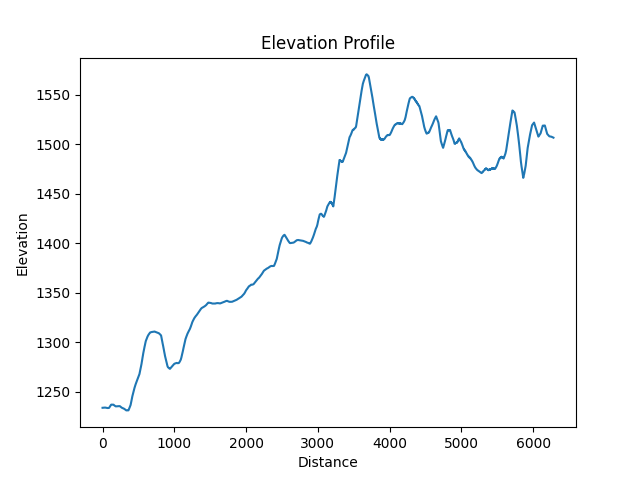
\includegraphics[width=0.5\linewidth]{elevation.png}
\caption{Plot over line \label{PlotOverCircularArcFigure}}
\end{figure}
\begin{block}{Acknowlegment}
I would like to thank \href{https://github.com/orgs/pyvista/teams/developers}{PyVista developer team} for developing useful library.
\end{block}
\begin{block}{References}
C. Bane Sullivan and Alexander Kaszynski, (2019). PyVista: 3D plotting and mesh analysis through a streamlined interface for the Visualization Toolkit (VTK). Journal of Open Source Software, 4(37), 1450, \url{https://doi.org/10.21105/joss.01450}
\end{block}
\begin{block}{Contact Information}
If you want to know pyvista more, join \href{http://slack.pyvista.org/}{Slack}.
\doclicenseThis
\end{block}
\end{textblock*}

\end{frame}
\end{document}

